% Options for packages loaded elsewhere
\PassOptionsToPackage{unicode}{hyperref}
\PassOptionsToPackage{hyphens}{url}
\PassOptionsToPackage{dvipsnames,svgnames,x11names}{xcolor}
%
\documentclass[
  letterpaper,
  DIV=11,
  numbers=noendperiod]{scrartcl}

\usepackage{amsmath,amssymb}
\usepackage{lmodern}
\usepackage{iftex}
\ifPDFTeX
  \usepackage[T1]{fontenc}
  \usepackage[utf8]{inputenc}
  \usepackage{textcomp} % provide euro and other symbols
\else % if luatex or xetex
  \usepackage{unicode-math}
  \defaultfontfeatures{Scale=MatchLowercase}
  \defaultfontfeatures[\rmfamily]{Ligatures=TeX,Scale=1}
\fi
% Use upquote if available, for straight quotes in verbatim environments
\IfFileExists{upquote.sty}{\usepackage{upquote}}{}
\IfFileExists{microtype.sty}{% use microtype if available
  \usepackage[]{microtype}
  \UseMicrotypeSet[protrusion]{basicmath} % disable protrusion for tt fonts
}{}
\makeatletter
\@ifundefined{KOMAClassName}{% if non-KOMA class
  \IfFileExists{parskip.sty}{%
    \usepackage{parskip}
  }{% else
    \setlength{\parindent}{0pt}
    \setlength{\parskip}{6pt plus 2pt minus 1pt}}
}{% if KOMA class
  \KOMAoptions{parskip=half}}
\makeatother
\usepackage{xcolor}
\usepackage[normalem]{ulem}
\setlength{\emergencystretch}{3em} % prevent overfull lines
\setcounter{secnumdepth}{-\maxdimen} % remove section numbering
% Make \paragraph and \subparagraph free-standing
\ifx\paragraph\undefined\else
  \let\oldparagraph\paragraph
  \renewcommand{\paragraph}[1]{\oldparagraph{#1}\mbox{}}
\fi
\ifx\subparagraph\undefined\else
  \let\oldsubparagraph\subparagraph
  \renewcommand{\subparagraph}[1]{\oldsubparagraph{#1}\mbox{}}
\fi


\providecommand{\tightlist}{%
  \setlength{\itemsep}{0pt}\setlength{\parskip}{0pt}}\usepackage{longtable,booktabs,array}
\usepackage{calc} % for calculating minipage widths
% Correct order of tables after \paragraph or \subparagraph
\usepackage{etoolbox}
\makeatletter
\patchcmd\longtable{\par}{\if@noskipsec\mbox{}\fi\par}{}{}
\makeatother
% Allow footnotes in longtable head/foot
\IfFileExists{footnotehyper.sty}{\usepackage{footnotehyper}}{\usepackage{footnote}}
\makesavenoteenv{longtable}
\usepackage{graphicx}
\makeatletter
\def\maxwidth{\ifdim\Gin@nat@width>\linewidth\linewidth\else\Gin@nat@width\fi}
\def\maxheight{\ifdim\Gin@nat@height>\textheight\textheight\else\Gin@nat@height\fi}
\makeatother
% Scale images if necessary, so that they will not overflow the page
% margins by default, and it is still possible to overwrite the defaults
% using explicit options in \includegraphics[width, height, ...]{}
\setkeys{Gin}{width=\maxwidth,height=\maxheight,keepaspectratio}
% Set default figure placement to htbp
\makeatletter
\def\fps@figure{htbp}
\makeatother

\KOMAoption{captions}{tableheading}
\makeatletter
\makeatother
\makeatletter
\makeatother
\makeatletter
\@ifpackageloaded{caption}{}{\usepackage{caption}}
\AtBeginDocument{%
\ifdefined\contentsname
  \renewcommand*\contentsname{Table of contents}
\else
  \newcommand\contentsname{Table of contents}
\fi
\ifdefined\listfigurename
  \renewcommand*\listfigurename{List of Figures}
\else
  \newcommand\listfigurename{List of Figures}
\fi
\ifdefined\listtablename
  \renewcommand*\listtablename{List of Tables}
\else
  \newcommand\listtablename{List of Tables}
\fi
\ifdefined\figurename
  \renewcommand*\figurename{Figure}
\else
  \newcommand\figurename{Figure}
\fi
\ifdefined\tablename
  \renewcommand*\tablename{Table}
\else
  \newcommand\tablename{Table}
\fi
}
\@ifpackageloaded{float}{}{\usepackage{float}}
\floatstyle{ruled}
\@ifundefined{c@chapter}{\newfloat{codelisting}{h}{lop}}{\newfloat{codelisting}{h}{lop}[chapter]}
\floatname{codelisting}{Listing}
\newcommand*\listoflistings{\listof{codelisting}{List of Listings}}
\makeatother
\makeatletter
\@ifpackageloaded{caption}{}{\usepackage{caption}}
\@ifpackageloaded{subcaption}{}{\usepackage{subcaption}}
\makeatother
\makeatletter
\@ifpackageloaded{tcolorbox}{}{\usepackage[many]{tcolorbox}}
\makeatother
\makeatletter
\@ifundefined{shadecolor}{\definecolor{shadecolor}{rgb}{.97, .97, .97}}
\makeatother
\makeatletter
\makeatother
\ifLuaTeX
  \usepackage{selnolig}  % disable illegal ligatures
\fi
\IfFileExists{bookmark.sty}{\usepackage{bookmark}}{\usepackage{hyperref}}
\IfFileExists{xurl.sty}{\usepackage{xurl}}{} % add URL line breaks if available
\urlstyle{same} % disable monospaced font for URLs
\hypersetup{
  pdftitle={Jonathan T. Oxborrow},
  colorlinks=true,
  linkcolor={blue},
  filecolor={Maroon},
  citecolor={Blue},
  urlcolor={Blue},
  pdfcreator={LaTeX via pandoc}}

\title{Jonathan T. Oxborrow}
\usepackage{etoolbox}
\makeatletter
\providecommand{\subtitle}[1]{% add subtitle to \maketitle
  \apptocmd{\@title}{\par {\large #1 \par}}{}{}
}
\makeatother
\subtitle{Analytics, Pricing, S\&OP, and Economics Professional}
\author{}
\date{}

\begin{document}
\maketitle
\ifdefined\Shaded\renewenvironment{Shaded}{\begin{tcolorbox}[boxrule=0pt, frame hidden, enhanced, interior hidden, borderline west={3pt}{0pt}{shadecolor}, breakable, sharp corners]}{\end{tcolorbox}}\fi

\begin{longtable}[]{@{}
  >{\centering\arraybackslash}p{(\columnwidth - 2\tabcolsep) * \real{0.2603}}
  >{\raggedright\arraybackslash}p{(\columnwidth - 2\tabcolsep) * \real{0.7397}}@{}}
\toprule()
\endhead
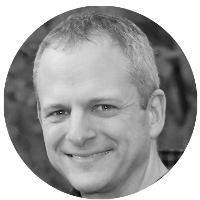
\includegraphics[width=1.04167in,height=\textheight]{assets/avatar.png}
& \begin{minipage}[t]{\linewidth}\raggedright
209 Court Drive

Washington, IL 61571

\href{mailto:jonathan.todd.oxborrow@gmail.com}{\nolinkurl{jonathan.todd.oxborrow@gmail.com}}
\end{minipage} \\
\bottomrule()
\end{longtable}

\hypertarget{social-links}{}
\begin{longtable}[]{@{}
  >{\centering\arraybackslash}p{(\columnwidth - 6\tabcolsep) * \real{0.2231}}
  >{\centering\arraybackslash}p{(\columnwidth - 6\tabcolsep) * \real{0.2417}}
  >{\centering\arraybackslash}p{(\columnwidth - 6\tabcolsep) * \real{0.2355}}
  >{\centering\arraybackslash}p{(\columnwidth - 6\tabcolsep) * \real{0.2955}}@{}}
\toprule()
\endhead
\href{mailto:jonathan.todd.oxborrow@gmail.com}{
\includegraphics[width=0.26042in,height=\textheight]{assets/envelope.png}}
&
\href{tel:309-822-2113}{
\includegraphics[width=0.26042in,height=\textheight]{assets/cell-phone.png}}
&
\href{https://www.linkedin.com/in/joxborrow1}{
\includegraphics[width=0.26042in,height=\textheight]{assets/linkedin-round.png}}
&
\href{http://github.com/joxborrow}{
\includegraphics[width=0.26042in,height=\textheight]{assets/github-icon-logo-png-transparent.png}} \\
\bottomrule()
\end{longtable}

\hypertarget{experience}{%
\subsection{\texorpdfstring{\textsc{\uline{Experience}}}{Experience}}\label{experience}}

\hypertarget{analytics-manager---parts-pricing}{%
\subsubsection{Analytics Manager - Parts
Pricing}\label{analytics-manager---parts-pricing}}

Manages a team of four Data Engineers and four Data Scientists providing
analytics and system support for the Global Aftermarket Parts Pricing
and Sales Variance Division. Responsible for managing analytics efforts
for aftermarket pricing efforts for XXX million dollars of annual
revenue. Fulfills the role of Data Steward for aftermarket parts pricing
data. Fulfills the role of IT owner for key pricing systems including
AWS, Snowflake, and new parts pricing system. Responsible supporting
corporate data governance and security efforts. Provides thought
leadership for

Primary responsibilities include automation and modernization of pricing
and sales variance processes, planning and directing analytics projects,
and recruiting and developing data science talent. Also, supporting and
leading key multi-year data efforts in the implementation of the a new
multi-million dollar pricing system.

\hypertarget{senior-analytics-team-lead}{%
\subsubsection{Senior Analytics Team
Lead}\label{senior-analytics-team-lead}}

Coordinates day to day Caterpillar Part Pricing Analytics activities and
task management using modern DevoOps tools. Supports pricing automation
efforts as well as pricing studies using the R language. Directly
responsible for pricing \$75 million in annual parts sales and over
150,000 individual part numbers. Provides programming support of data
engineering efforts in PySpark. Experienced creating analytic apps and
dashboards with Alteryx and Tableau respectively. Coordinates parts
pricing project efforts and supports personnel and resource management.

\hypertarget{sop-coordinator---analytics}{%
\subsubsection{S\&OP Coordinator -
Analytics}\label{sop-coordinator---analytics}}

Led data efforts for new forecasting system implementation. Prepared
first centralized Energy \& Transportation scoped hierarchical
statistical forecast. Engineered first industry standard forecast
accuracy metric for Energy \& Transportation. Managed setup of Energy \&
Transportation S\&OP analytics server.

\hypertarget{machine-demand-forecaster}{%
\subsubsection{Machine Demand
Forecaster}\label{machine-demand-forecaster}}

Prepared the Demand Forecast and Long Term Forecast for mining product.
Forecasted over \$3 billion in annual revenue. Mined Haver databases for
leading indicators. Used these indicators in a machine learning model
for mining industry sales. Developed Excel based forecasting tool for
the division.

\hypertarget{regional-economic-analyst}{%
\subsubsection{Regional Economic
Analyst}\label{regional-economic-analyst}}

Prepared the North America economic forecast proposal, including GDP,
inflation, interest rate, construction and mining activity forecasts.
Also prepared North American machine industry sales forecast. Supported
the company business cycle monitoring processes.

\hypertarget{senior-economic-analyst}{%
\subsubsection{Senior Economic Analyst}\label{senior-economic-analyst}}

Provided economic forecast proposal for the United States and Canada.
Enhanced the U.S. GDP forecast through the use of chaining to ensure
hierarchical forecast consistency. Authored Canada economic summary for
Board of Directors meetings.

\hypertarget{economic-analyst}{%
\subsubsection{Economic Analyst}\label{economic-analyst}}

Maintained Latin America databases and monthly business processes.
Provided translation of relevant Spanish language news material.
Assisted in the preparation of written economic assumption reports for
Business Plan and Long Term forecast.

\hypertarget{senior-quantitative-analyst}{%
\subsubsection{Senior Quantitative
Analyst}\label{senior-quantitative-analyst}}

Responsible for the maintaining databases and monthly processes for Asia
Pacific and Latin America. Assisted elsewhere as necessary.

\hypertarget{education}{%
\subsection{\texorpdfstring{\textsc{\uline{Education}}}{Education}}\label{education}}

\hypertarget{m.a.-economics}{%
\subsubsection{M.A.~Economics}\label{m.a.-economics}}

\begin{description}
\item[Illinois State University (May 2005)]
Received a M.A.~in Economics with a GPA of 3.41. Coursework included an
above average load of econometrics, statistics, and labor economics
coursework. The Master of Arts degree required demonstration of the
command of a foreign language.
\end{description}

\hypertarget{b.a.-economics}{%
\subsubsection{B.A. Economics}\label{b.a.-economics}}

\begin{description}
\item[Brigham Young University (December 2002)]
Received a B.A. in Economics with a GPA of 3.19. Coursework included a
number courses in mathematics, computer programming, and Spanish.
Bachelor of Arts required additional mathematics.
\end{description}

\hypertarget{certifications}{%
\subsection{\texorpdfstring{\textsc{\uline{Certifications}}}{Certifications}}\label{certifications}}

\hypertarget{professional-forecaster}{%
\subsubsection{Professional Forecaster}\label{professional-forecaster}}

\begin{description}
\item[Institute of Business Forecasting and Planning (June 2010 - June
2014)]
Earned the designation of Certified Professional Forecaster from the
Institute of Business Forecasting and Planning (IBF).
\end{description}

\hypertarget{economic-measurement}{%
\subsubsection{Economic Measurement}\label{economic-measurement}}

\begin{description}
\item[National Association for Business Economics (October 2011)]
Earned the Certificate in Economic Measurement from the National
Association for Business Economics (NABE).
\end{description}

\hypertarget{core-proficiencies-skills}{%
\subsection{\texorpdfstring{\textsc{\uline{Core Proficiencies \&
Skills}}}{Core Proficiencies \& Skills}}\label{core-proficiencies-skills}}

\hypertarget{leadership}{%
\subsubsection{Leadership}\label{leadership}}

\begin{longtable}[]{@{}
  >{\raggedright\arraybackslash}p{(\columnwidth - 0\tabcolsep) * \real{1.0112}}@{}}
\toprule()
\endhead
\begin{minipage}[t]{\linewidth}\raggedright
\begin{itemize}
\tightlist
\item
  Communication ‐ Demonstrated strong communicator, both verbal and
  written.
\item
  Ownership ‐ See things through. Takes responsibility for outcomes.
\item
  Integrity ‐ Honest, consistent, fair, driven by principles.
\item
  Teamwork ‐ Functions well as part of a team, both as lead or team
  member.
\item
  Goal/Result Oriented ‐ Sets goals, prioritizes activities to achieve
  best outcomes.
\item
  Continuous Learner ‐ Always investigating job relevant emerging
  technologies.
\end{itemize}
\end{minipage} \\
\bottomrule()
\end{longtable}

\hypertarget{analytics-productivity}{%
\subsubsection{Analytics \& Productivity}\label{analytics-productivity}}

Programming Languages \& Software

\begin{longtable}[]{@{}
  >{\raggedright\arraybackslash}p{(\columnwidth - 0\tabcolsep) * \real{1.0125}}@{}}
\toprule()
\endhead
\begin{minipage}[t]{\linewidth}\raggedright
\begin{itemize}
\tightlist
\item
  Proficient: R, RMarkdown, SQL, git, and MSOffice/VBA.
\item
  Experienced: Tableau, Python/Pyspark, SAS, STATA, EViews, shell
  scripting.
\item
  Functional: Power Automate, Office Script, Javascript, C/C++, docker
\end{itemize}
\end{minipage} \\
\bottomrule()
\end{longtable}

Statistics \& Analytics

\begin{longtable}[]{@{}
  >{\raggedright\arraybackslash}p{(\columnwidth - 0\tabcolsep) * \real{1.0112}}@{}}
\toprule()
\endhead
\begin{minipage}[t]{\linewidth}\raggedright
\begin{itemize}
\tightlist
\item
  Proficient: Time Series Modeling \& Forecasting, Seasonal Adjustment,
  Regression/GLM
\item
  Experienced: Classification, Simulation, Machine Learning, Survival
  Analysis
\item
  Functional: Network Analysis
\end{itemize}
\end{minipage} \\
\bottomrule()
\end{longtable}

\hypertarget{language}{%
\subsubsection{Language}\label{language}}

Reads, writes, and speaks Spanish. Lived in Chile for two years from
February of 1997 to February of 1999. Took Spanish coursework and
proficiency exams while in college.

English Native.

\hypertarget{additional-projects-activities}{%
\subsection{\texorpdfstring{\textsc{\uline{Additional Projects \&
Activities}}}{Additional Projects \& Activities}}\label{additional-projects-activities}}

\hypertarget{ynabr}{%
\subsubsection{\texorpdfstring{\href{http://joxborrow.github.io/ynabr}{YNABR}}{YNABR}}\label{ynabr}}

This github project is an API client package for the
\texttt{You\ Need\ a\ Budget} web application for downloading data. It
is implemented in the R programming language.

\hypertarget{xrandrgui}{%
\subsubsection{\texorpdfstring{\href{https://github.com/joxborrow/xrandrgui}{XRANDRGUI}}{XRANDRGUI}}\label{xrandrgui}}

This github project is an experimental GUI for the xrandr Linux
commandline utility, implemented in Python.

\hypertarget{byu-idaho}{%
\subsubsection{\texorpdfstring{\href{http://www.byui.edu}{BYU-Idaho}}{BYU-Idaho}}\label{byu-idaho}}

Online Instructor - Econ 150: Microeconomics, Fall 2021 - present.



\end{document}
